%% template for IEICE Transactions
%% v2.1 [2015/10/31]
\documentclass[paper]{ieice}
%\documentclass[invited]{ieice}
%\documentclass[position]{ieice}
%\documentclass[survey]{ieice}
%\documentclass[invitedsurvey]{ieice}
%\documentclass[review]{ieice}
%\documentclass[tutorial]{ieice}
%\documentclass[letter]{ieice}
%\documentclass[brief]{ieice}
%\usepackage[dvips]{graphicx}
%\usepackage[pdftex]{graphicx,xcolor}
\usepackage[dvipdfmx]{graphicx,xcolor}
\usepackage[fleqn]{amsmath}
\usepackage{newtxtext}
\usepackage[varg]{newtxmath}

\setcounter{page}{1}
%\breakauthorline{}% breaks lines after the n-th author

\field{D}
%\SpecialIssue{}
%\SpecialSection{}
%\theme{}
\title{Rogue Access Point Detection by Using ARP Failure under the MAC Address Duplication}
%\title[title for header]{title}
%\titlenote{}
\authorlist{
\authorentry[igarashi@sasase.ics.keio.ac.jp]{Kosuke Igarashi}{n}{keio}\MembershipNumber{}
\authorentry[kato@sasase.ics.keio.ac.jp]{Hiroya Kato}{s}{keio}\MembershipNumber{1722956}
\authorentry[sasase@ics.keio.ac.jp]{Iwao Sasase}{f}{keio}\MembershipNumber{7908862} % keio $B$O%i%Y%k(B
}
\affiliate[keio]{Dept. of Information and Computer Science, Keio University\\ 3-14-1 Hiyoshi, Kohoku, Yokohama, Kanagawa 223-8522, Japan}
%\paffiliate[present affiliate label]{Presently, the author is with the }

\received{2015}{1}{1}
\revised{2015}{1}{1}

%% <local definitions here>
%target AP
\newcommand{\SSID}{\rm SSID_{connect}}
\newcommand{\tarAP}{\rm AP_{connect}}
\newcommand{\tarMAC}{m_{\rm connect}}
%client
\newcommand{\userMAC}{m_{\rm user}}
%input AP
\newcommand{\inputAP}{\rm AP_{owner}}
\newcommand{\inputMAC}{m_{\rm input}}
%MAC address in sbxt
\newcommand{\stba}{m_{\rm a}}
\newcommand{\stbA}{m_{\rm A}}
\newcommand{\stbb}{m_{\rm b}}
\newcommand{\stbB}{m_{\rm B}}
%% </local definitions here>

\begin{document}
\maketitle
\begin{summary}
Detecting a Rouge Access Point (RAP) in Wi-Fi network is imperative.
The previous scheme is user side detection focusing on two channels used by a RAP.
That scheme can detect a RAP in stable traffic environment by revealing the channel used with a Legitimate Access Point (LAP) with intentional interference.
However, the detection performance is degraded in the real environment where traffic is more unstable because it affects the traffic on the channel.
Thus, it is necessary to design the scheme which is independent of such factors.
In this paper, we propose RAP detection by using Address Resolution Protocol (ARP) failure under the Media Access Control (MAC) address duplication.
Our main idea is that the traffic is relayed via a RAP and a LAP on the LAN path between a client and a gateway under the attack.
This is because the RAP must be established between a client and a LAP to provide Internet connection.
On the basis of this idea, the proposed scheme reveals that the Access Point (AP) with whih a client connects is a RAP by discovering the MAC address of a LAP on the path.
In order to find the MAC address, we leverage the phenomenon that a client cannot receive ARP reply packets in the situation where its MAC address and that of a AP are duplicated on the path.
By doing this, the presence of a LAP is revealed, which can judge that the connected AP is a RAP.
In our evaluation, the proposed scheme achieves accuracy of 96.5\% even in unstable traffic environment.
True positive rate and false positive rate are 31.0\% higher and 9.0\% lower than the previous scheme.
Furthermore, the proposed scheme can detect RAPs accurately in real environment where the previous scheme cannot.
\end{summary}
\begin{keywords}
Evil Twin Attack, Rogue Access Point, Address Resolution Protocol
\end{keywords}

\section{Introduction}
With the rapid development of wireless communication techniques, Wi-Fi is deployed as the most commonly used Internet access technology and keeps spreading all over the world\cite{bg-evi}.
It is located in everywhere of our daily life, such as shopping malls, restaurants, public transit systems and so on.
While the free access to Wi-Fi network attracts a large number of users, it also allows adversaries to launch attacks against the users just by setting up a Rogue Access Point (RAP) on their laptop in the network, which is called ``Evil Twin Attack (ETA) ''\cite{laptop-evi}.
The RAP clones the Service Set IDentifier (SSID) and even Media Access Control (MAC) address of a Legitimate Access Point (LAP) provided by a public facility, which is the reason why it is called ETA.
In particular, cloning SSID enables adversaries to make clients connect with a RAP because wireless devices connect automatically to an Access Point (AP) which has the strongest Received Signal Strength Indication (RSSI) among all APs with the same SSID.
In the ETA, a RAP is established between a client and the Internet as Man-In-The-Middle (MITM) attacks \cite{spoof-evi}.
Thus, adversaries can eavesdrop on the exchange of sensitive information such as identity credentials, and bank accounts by observing relayed packets through their laptop between a client and a LAP.
In addition, adversaries can also carry out an active attack by leading a user to phishing websites or infecting a client with malicious softwares\cite{research}.
By exploiting the characteristic that users freely connect free Wi-Fi network,  an adversary can succed in the attacks without being noticed by a user.
Thus, the detection of the RAPs is urgent demand.

The attack model is divided into two models based on how a RAP provides the Internet service to client.
The one is a model where a RAP uses mobile communication.
However, it can be easily detected with Internet Services Provider (ISP) names or Global IP addresses\cite{rtt}.
Thus, we focus on the other model where a RAP uses the same gateway with LAPs in the network by directly connecting with one of them since it cannot be easily detected by existing schemes.

Exisiting RAP detection schemes supposing this attack model are divided into network administrator side detections and user side detections.
The network administrator side detections mainly use whitelist-based mechanisms based on fingerprints of APs\cite{prapd}, \cite{clockskew}.
However, those solutions are inapplicable to Wi-Fi hotspots since they make network administrators set additional costly devices in their infrastructures.
On the other hand, the user side detections focus on characteristics in packet transmission.
In particular, most of the exisiting schemes utilize network latency, such as Round-Trip Time (RTT) or Inter-packet Arrival Time \cite{rtt}, \cite{iat}.
However, since such delay is caused by the software-based RAP on a laptop, latency based schemes can be easily evaded by using a hardware-based RAP.
Thus, in order to cope with both software-based RAPs and hardware-based ones, the user side detection scheme which focuses on two communication channels used by a RAP has been proposed \cite{previous}.
That scheme can detect the RAP by finding out these two channels on the basis of the decline in the throughput.
That scheme is the most useful detection since it can deal with a hardware-based RAP which does not cause delay.
Hence, we focus on that scheme \cite{previous} as the previous scheme.
Although the previous scheme is successful in the experimental environment, its detection performance is degraded by unstable traffic in real environment.
Therefore, it is necessary to realize the user side detection which is independent of the network traffic.

In order to realize the user side detection which is independent of network traffic, in this paper, we propose RAP detection by using Address Resolution Protocol (ARP) failure under the MAC address duplication.
The main idea of the proposed scheme is that the traffic is relayed via two APs, namely the RAP and a LAP, on the LAN path from a client to a gateway.
Therefore, besides the connected RAP, a LAP exists inevitably on the other side of the RAP because of the MITM attack in an attack scenario.
On the basis of this idea, the proposed scheme reveals a connected AP as a RAP by finding MAC address of such a LAP from obtainable beacon frames by a client \cite{beacon}.
In order to find the MAC address, we leverage the phenomenon that a client cannot receive ARP reply packets from a gateway in the situation where there exists the duplicated MAC address, which is set in the packets as the destination address, on the path back to the client.
The proposed scheme intentionally creates such situation by setting the MAC address of a client to that of the LAP on the other side of the connected RAP.
By doing this, the proposed scheme can reveal the connected AP as a RAP regardless of network traffic.
The contributions of the proposed scheme are as follows:
\begin{enumerate}
    \renewcommand{\labelenumi}{\arabic{enumi}).}
    \item To the best of our knowledge, the proposed scheme is the first one which is independent of fingerprints of a RAP. By focusing only on the characteristic of attack and a MAC address of a LAP, the proposed scheme does not allow an adversary to avoid detection by manipulating features of the RAP.
    \item The proposed scheme achieves accurate detection without any error even in real LAN traffic. It can guarantee beneficial effects on every available hotspot.
\end{enumerate}
The rest of this paper is constructed as follows: Related works are described in Section \ref{sec:2}.
The attack model, previous scheme and its shortcoming are introduced in Section \ref{sec:3}.
The proposed scheme is explained in Section \ref{sec:4}.
Various evaluation results are shown in Section \ref{sec:5}.
Finally, the conclusions of this paper are presented in Section \ref{sec:6}.

\section{Related Works}\label{sec:2}
RAP detection schemes are mainly classified into two categories: network administrator side detections and user side detections.
Network administrator side detections \cite{prapd}, \cite{clockskew} focus on the fingerprints of an AP such as RSSI and clock skew which cannot be spoofed by an adversary.
A RAP can be detected by comparing its fingerprints with those in the predefined whitelist collected by equipments such as traffic sensors in each Wi-Fi network.

Wu et al. \cite{prapd} focus on the RSSI which is hard to be forged arbitrarily and highly correlated to a location of an AP and its power.
For each LAP in a network, RSSI, which is measured by additional costly devices, is registered in a whitelist beforehand.
By using RSSI, even if the MAC address is spoofed by adversary, that scheme can disclose that it is a RAP at a different location from that of LAPs.
However, that scheme is hard to detect a RAP which is located near the LAP because RSSI is not as exact as it can indicate a small difference of the nearby location.
Although RSSI is useful as a supplementary feature, using only RSSI is insufficient to detect a RAP with high accuracy.

In order to detect in more detail, Lanze et al. \cite{clockskew} focus on clock skew as a device fingerprinting based purely on physical properties.
Clock skew is the time gap of clock signals caused by the crystal oscillator, which is one of the components equipped in each AP.
Since the clock skew is a precise feature which is unique to each AP, that scheme can be useful.
However, that scheme is inapplicable to Wi-Fi hotspots because it requires additional costly sensors for observing the feature.
%Administrators are required to set up additional devices in their infrastructures.
Thus, the detection schemes that require no equipment of additional devices by a network administrator are desired.

Meanwhile, user side detections \cite{rtt}, \cite{previous} do not need to introduce additional devices to a Wi-Fi hotspot.
They focus on differences in the packet transmission caused by the extra hop to a RAP on the path between a LAP and a client.
Compared with legitimate networks, extra hop results in several measurable changes in LAN communication such as RTT and channel used between a client and DNS server.

Mustafa et al. \cite{rtt} differentiate RAPs from LAPs by measuring the RTT between the client and the DNS server through a AP or APs.
Because there exists the extra hop caused by the RAP on the path, RTT is longer than that in the case where a client directly connects to the LAP.
Although that scheme is useful only for the case where the adversary sets a RAP up on the laptop, Jang et al. \cite{previous} reveal the fact that the computational power of the software bridging mainly accounts for the packet delay.
Thus, the adversary can evade the detection based on packet delay by utilizing hardware-based RAPs having little bridging delay unlike software-based RAPs.

In order to detect both types of RAPs, namely, software-based and hardware-based ones, Jang et al. focus on two communication channels utilized by a RAP between a client and LAP\cite{previous}.
Whereas a RAP intervenes between a client and a LAP, two distinct channels are used.
This is because a RAP can be detected by \cite{rtt} because of latency caused by the channel interference if the same channel is used in the both paths.
For example, it is assumed that channel 1 is used as the channel between a client and a RAP, and channel 6 is that between the RAP and a LAP.
That scheme detects the RAP by finding out the presence of these two distinct channels with the throughput of the transmission from the client to the DNS server.
That scheme is the most robust user side detection which is independent of the performance of the RAP because it is the countermeasure against a reasonable attack model where the hardware-based RAP is used.
Thus, we select the scheme \cite{previous} as the previous scheme and elaborate it in the next section.
%In the next section, we elaborate the previous scheme.

\section{Attack Model and Previous Scheme}\label{sec:3}
\begin{figure}[t]
    \begin{center}
        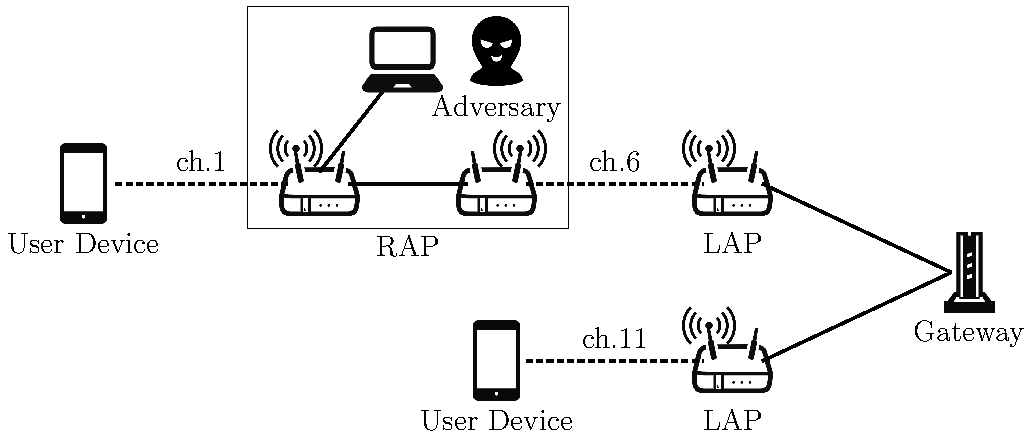
\includegraphics[scale=0.48]{attack-model/attack-model.pdf}
        \caption{The Attack Model}
        \label{fig:model}
    \end{center}
\vspace{-2zh}
\end{figure}
\subsection{Attack Model}
In an ETA, the adversary sets up a RAP using a SSID of a LAP in the targeted Wi-Fi network.
Besides, in some cases, the MAC address of the RAP is cloned from one of the LAPs in the network\cite{spoof-evi}.
As a result, although a client receives SSID broadcast from the RAP and LAPs, it cannot differentiate between them.
The RAP sends beacon frames with stronger signals since the client simply connects with the AP that has a higher RSSI.
\figurename~\ref{fig:model} shows the attack model, where a RAP relays traffic via a LAP as a MITM attack to eavesdrop client's sensitive data.
%Since MITM attack does not succeed in protected Wi-Fi\cite{kataoka}, whose LAPs have security protocol such as WPA2, it is beyond the scope of our work.
%Thus, the targeted network is open Wi-Fi in the model.
In our model, the targeted network is open Wi-Fi, whose LAPs have no security protocols such as WPA2, since MITM attack does not succeed in a protected Wi-Fi\cite{kataoka}.
%Thus, protected Wi-Fi is beyond the scope of our work.
By using the same gateway with the LAN, the adversary can evade simple detections with ISP names or Global IP addresses \cite{rtt}.
In addition to that, the adversary in our model exploits a hardware-based AP, which is introduced by \cite{previous}, in order to realize a detection scheme independent of its computational performance.
The distinct channels can be used on the both sides to avoid channel interference since the RAP is composed of two APs which are interconnected with a LAN cable.
One of these routers is connected to a LAP in station mode, and the other disguise client as a LAP in service mode.
Because a high-end router which can relay traffic with distinct channels appears nowadays, it can replace a RAP in our model.

\subsection{Previous Scheme}
\subsubsection{Overview of the Previous Scheme}
The main idea of the previous scheme \cite{previous} is that the adversary needs to use two distinct channels on the path from a client to the gateway to avoid channel interference each other.
The one is the channel for the path between a LAP and a RAP, and the other is that for the path between a RAP and the client.
Thus, from the perspective of the client, there exists another channel on the route which is different from the channel using with the connected AP.
The extra channel cannot be observed directly from the client.
The previous scheme detects the RAP by finding out this second channel on the basis of the decline in the throughput.
In order to decrease the throughput, the previous scheme saturates the channel used between a LAP and the RAP by intentionally interfering with an additional equipment in a client.
For example, when a client is using channel 1 with the connected AP whose benignancy is unidentified, the equipment in a client transmits a large number of packets to all the channel except channel 1 to saturate traffic on the path.
If there exists the other channel on the route, the decline in the throughput can be observed by the client, and the presence of the RAP is revealed.

\subsubsection{Shortcoming of the Previous Scheme}\label{sec:shortcoming}
%\begin{figure}[t]
%   \begin{center}
%      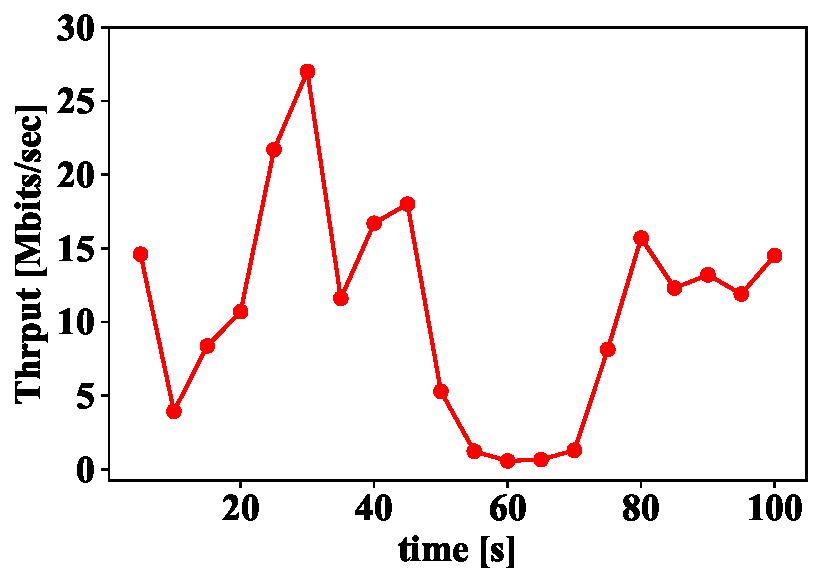
\includegraphics[scale=0.3]{figure/Thrput.pdf}
%     \caption{Throughput in a Cafe}
%    \label{thrput}
%    \end{center}
%   \vspace{-2zh}
%\end{figure}
\begin{table}[t] 
    \begin{center}
        \caption{The Accuracy in Different Traffic Environment}
        \label{tab:thrput result}
        \begin{tabular}{c c} \hline
            Constant Traffic (80Mbps) & Random Traffic \\ \hline \hline
            0.920 & 0.765 \\ \hline
        \end{tabular}
    \end{center}
    \vspace{-2zh}
\end{table}
Although the previous scheme is successful in the detection for a hardware-based RAP in the experimental environment, it cannot accurately detect the RAP in the real world.
This is because throughput is considerably dependent on various factors of the network environment such as mobility of the traffic, collisions, network topology changes, and unintentional interference.
%\figurename~\ref{thrput} shows the graph regarding the change of throughput in a cafe on a weekday.
%As shown in \figurename~\ref{thrput}, since the traffic in real environment is unsteady in fact, the previous scheme is subject to environmental changes, which can lead to degrade the detection performance.
\tablename~\ref{tab:thrput result} shows the detection accuracy in different traffic environment.
The one is the constant traffic environment, where the 80Mbps traffic is communicated through the LAP, and the other is the random traffic environment, which reproduces the real LAN in our lives.
In the former environment, the previous scheme can detect with high accuracy.
On the contrary, it is degraded to 0.765 in random traffic.
The previous scheme is subject to traffic environment, which can lead to degradation of the detection performance.
Thus, the requirement that we must satisfy is to leverage factors which are independent of the network traffic.

\section{Proposed Scheme}\label{sec:4}
In order to meet the requirements mentioned in Section \ref{sec:shortcoming}, in this paper, we propose RAP detection by using ARP failure under the MAC address duplication.
In the following subsections, we explain the idea and the algorithm in detail.

\subsection{Idea}
The main idea of the proposed scheme is that the traffic is relayed via two APs, namely, the RAP and LAP, on the path from a client to a gateway.
In general, a LAP is the only device which exists on the path.
Therefore, in this case, the LAP is identical to the AP directly connected with a client.
In an attack scenario, besides the connected AP, a LAP exists inevitably on the other side of the AP.
Therefore, a connected AP can be revealed as the RAP when the presence of a LAP is detected on the other side of it.

On the basis of this idea, the proposed scheme reveals a LAP exists on the other side of the connected AP by finding out its MAC address.
In order to discover the MAC address of such LAP, we leverage the phenomenon that a client cannot receive ARP reply packets in the situation where there exist duplicate MAC addresses on the path from a gateway back to a client.
The proposed scheme intentionally creates such situation by setting the MAC address of a client to the MAC addresses obtained from beacon frames of APs in its communication range.
Note that the MAC address of the AP with which a client connects directly is excluded from targets for setting MAC addresses.
If the MAC address of a client is set to that of a LAP on the other side of the connected AP, the LAP receives ARP reply packets whose original destination is the client before the client receives them.
Thus, since the client cannot receive ARP reply packets, it continues to resend ARP requests, which results in disabling internet connectivity.
By observing the continuance of resending ARP request packets within a definite period of time without ARP reply packets, the proposed scheme can reveal that there exists the RAP and LAP on the path, which detects the attack. %reply $B$,Mh$k$^$GAw$jB3$1$^$9(B

When a client connects with the RAP, there exists a MAC address of a LAP in the communication range of a client.
This is because the RAP must be located relatively near a LAP to avoid communication delay.
Hence, we can inevitably obtain the MAC address of a LAP in the case where the RAP exists in a network.
%---------------------------------------------------------------------------------------------------------------SSID$B$N8BDj$K$h$k8uJd$N9J$j9~$_$K$D$$$F!J=$@5!K(B
At this time, in addition, only the MAC addresses of APs which have the SSID used in the targeted network are collected since a RAP clones its SSID to deceive clients.
By doing this, more efficient detection is realized since we can exclude irrelevant LAPs in its communication range in a real situation.
%---------------------------------------------------------------------------------------------------------------SSID$B$N8BDj$K$h$k8uJd$N9J$j9~$_$K$D$$$F!J85!9!K(B
%In the real situation, it is possible that there exist several LAPs in a communication range of a client.
%Thus, we collect the only MAC addresses of APs which have the SSID used in targeted network.
%This is because a RAP must utilize an SSID of a LAP for pretending to be a LAP.
%---------------------------------------------------------------------------------------------------------------$BJ#?t(BLAP$B$N>u67$K$D$$$F!J=$@5!K(B
Furthermore, even if multiple LAPs which have the same SSID, and a RAP are set in the targeted LAN as in real situations, the proposed scheme can detect without any problem.
In that case, only a client which forms MITM topology with a RAP cannot receive ARP replies.
Because ARP replies can be sent to all of the LAPs with the duplicated addresses, the other LAPs which do not connect with the RAP can get the replies \cite{kataoka}.
Thus, the connectivity of each LAP is kept available as usual.
Also, the other clients which directly connet with the LAP can use Internet as usual without being attacked since they do not form MITM with the RAP.
%Thus, it means it can detect in the case that MITM attacks are formed the detec
%---------------------------------------------------------------------------------------------------------------$BJ#?t(BLAP$B$N>u67$K$D$$$F!J85!9!K(B
%A client can receive ARP reply packets even if its MAC address is set to that of each LAP via which the traffic is not relayed to a gateway.
%This is because the packets can be sent to both client and each LAP.
%---------------------------------------------------------------------------------------------------------------
Since the proposed scheme is independent of various factors of the real LAN environment, it is useful for overcoming the shortcoming of the previous scheme.
In addition, the proposed scheme is not affected by a spoofed MAC address because it focuses on the only legitimate MAC address never spoofed.

\subsection{Algorithm} \label{sec:alg}
\begin{figure}[t]
    \begin{center}
        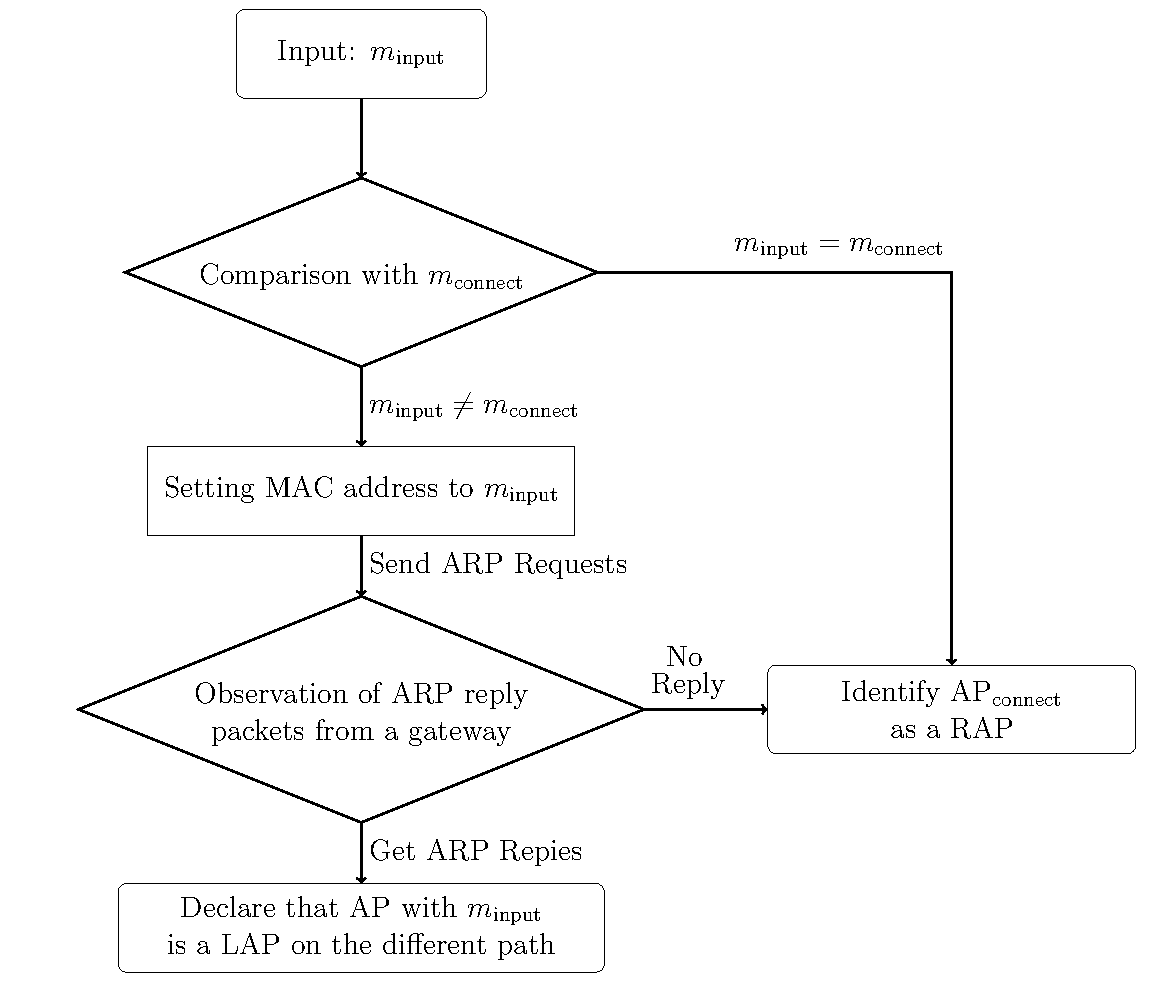
\includegraphics[scale=0.43]{flowchart/flowchart.pdf}
        \caption{The Flowchart of the Proposed Scheme}
        \label{fig:flowchart}
    \end{center}
\vspace{-2zh}
\end{figure}
In this subsection, the algorithm of the scheme is explained.
Its goal is to reveal whether the connected AP is a LAP or not, namely $\tarAP = LAP$ or $\tarAP \ne LAP$, by searching the MAC address of a LAP between a client and a gateway.
$\tarAP$ denotes a AP which connects with a client.
The algorithm mainly consists of 1) MAC address collection and 2) ARP reply based detection.

\subsubsection{MAC Address Collection}
Let $\SSID$ and $\tarMAC$ denote SSID and MAC address of $\tarAP$, respectively.
The set of MAC addresses of APs whose SSID is identical to $\SSID$  is created with beacon frames of them.
Let the set is denoted by $M_{\rm all}=\{m_{\rm i nput}|0\le input \le n_{\rm al l}  \}$, where $n_{\rm all}$ is the number of collected MAC addresses.

\subsubsection{ARP Reply based Detection}
\figurename~\ref{fig:flowchart} shows the flowchart of this phase.
This phase consists of three procedures which are a) Comparison with $\tarMAC$, b) Setting MAC address, and c) Observation of ARP reply from the gateway to the client.
These procedures are repeatedly conducted for every $\inputMAC$  in $M_{all}$ unless the RAP is detected.

In the first phase, $\inputMAC$ and $\tarMAC$ are compared.
If they are the same MAC address, it easily judges that $\tarMAC$ is the cloned address.
In this case, the RAP is detected in the targeted LAN and the detection is finished since it is not the case in non attack scenario.
However, in the case where the RAP clones a MAC address of a LAP beyond the communication range of a client or it does not clone, it cannot be detected by this procedure by the accordance of its MAC address.
Thus, the process proceeds to the second phase.

In the second phase, the MAC address of a client is set to $\inputMAC$.
After that, the connection between the client and $\tarAP$ is once lost since the gateway becomes unable to use the original MAC address as a destination for the packets.
Thus, the client sends ARP request in order to reconnect with it through the $\tarAP$ automatically.

Finally, in the third procedure, the ARP reply packets whose destination is set as $\inputMAC$ are observed to investigate whether the AP with $\inputMAC$ is on the other side of $\tarAP$.
If the packets do not reach the client, the $\tarAP$ can be revealed as the RAP which exists between the client and the LAP with $\inputMAC$, and the detection phase is finished.
Otherwise, the benignancy of the $\tarAP$ still cannot be judged by the AP with $\inputMAC$.
In this case, the same procedures in the flowchart are repeatedly conducted for another $\inputMAC$ in $M_{A_{\rm all}}$ until the RAP is detected.
If the detection phase is carried out for all $\inputMAC$ without the detection of a RAP, the $\tarAP$ is declared as a LAP.
\begin{figure*}[ht]
    \begin{minipage}{0.33\hsize}
        \begin{center}
            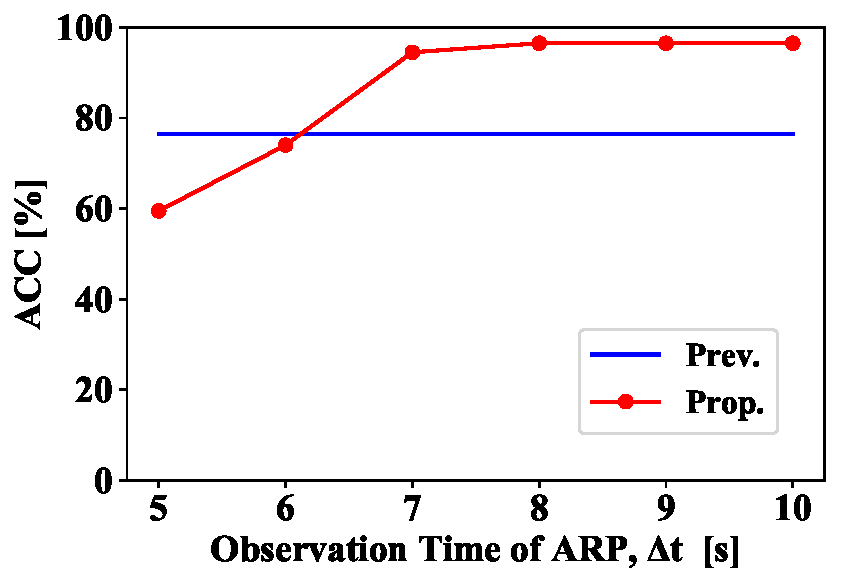
\includegraphics[scale=0.34]{figure/ACC.pdf}
        \end{center}
        \caption{The Avg. ACC of the Prop. and Prev.}
        \label{fig:acc}
    \end{minipage}
        \begin{minipage}{0.33\hsize}
        \begin{center}
            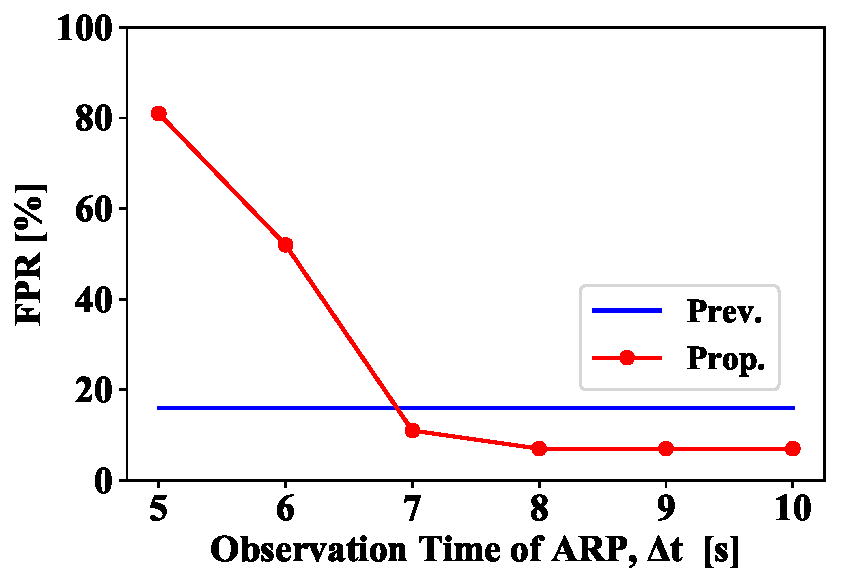
\includegraphics[scale=0.34]{figure/FPR.pdf}
        \end{center}
        \caption{The Avg. FPR of the Prop. and Prev.}
        \label{fig:fpr}
    \end{minipage}
    \begin{minipage}{0.33\hsize}
        \begin{center}
            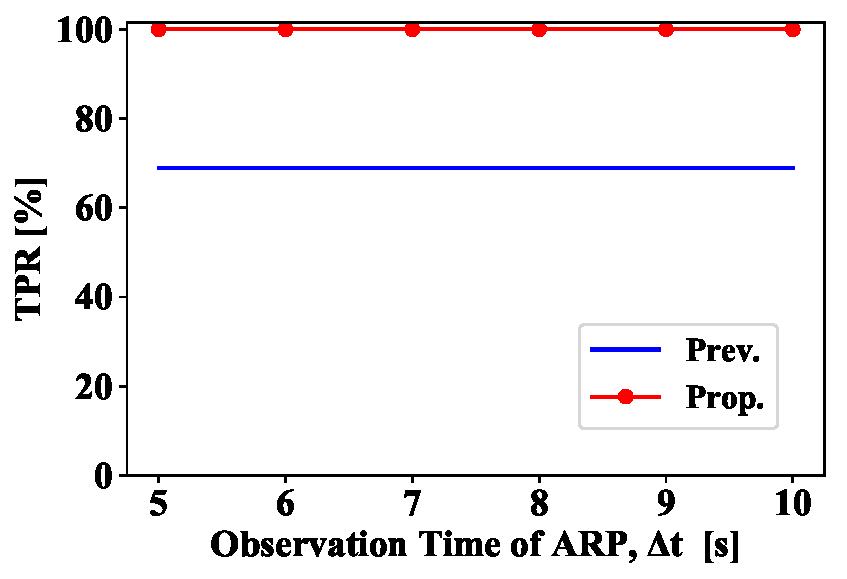
\includegraphics[scale=0.34]{figure/TPR.pdf}
        \end{center}
        \caption{The Avg. TPR of the Prop. and Prev.}
        \label{fig:tpr}
    \end{minipage}
\vspace{-1zh}
\end{figure*}
\section{Evaluation}\label{sec:5}
In order to demonstrate the effectiveness of the proposed scheme, we compare it with the previous scheme \cite{previous} which interferes the channel between a LAP and a RAP.

The metrics of the evaluation are ACCuracy (ACC), True Positive Rate (TPR), and False Positive Rate (FPR) defined as
\begin{gather}
    \mathrm{ACC} = \frac{\mathrm{TP} + \mathrm{TN}}{\mathrm{TP} + \mathrm{TN} + \mathrm{FP} + \mathrm{FN}}\\
    \mathrm{TPR} = \frac{\mathrm{TP}}{\mathrm{TP} + \mathrm{FN}}\\
    \mathrm{FPR} = \frac{\mathrm{FP}}{\mathrm{FP} + \mathrm{TN}}
\end{gather}
where TP, TN, FP, and FN denote the number of True Positive (RAPs are regarded as RAPs), True Negative (LAPs are regarded as LAPs), False Positive (LAPs are regarded as RAPs), and False Negative (RAPs are regarded as LAPs), respectively.
We evaluate the proposed scheme with these metrics in two scenarios which are the case of attack where a client connects with a RAP and that of non-attack where a client connects with a LAP.

\subsection{Experimental Setup}
\subsubsection{Detector}
We implemented the detectors in a laptop, which is a MacBook Pro with an Intel Core i5 CPU.
We observe ARP packets with T-shark, which is a tool for capturing packets\cite{wire}.
Besides, in order to reproduce the detection model in the previous scheme \cite{previous}, we use a TP-Link Archer C6 as an interference device.

\subsubsection{LAP and RAP}
TP-Link Archer C6 is also used to setup the LAP.
As regards the RAP, in order to use distinct channels on both sides as the model in the previous scheme, it is composed of two APs (TP-Link Archer C6 and TP-Link Archer C50).
These two APs, where one is in the station mode ($\rm AP_{sm}$) and the other is in AP mode ($\rm AP_{am}$), are interconnected using a LAN cable.
The $\rm AP_{sm}$ is responsible for repeating packets to and from the LAP, and the $\rm AP_{am}$ has a spoofed SSID.
All devices are operated in the IEEE 802.11n mode with MIMO.
We arrange a LAP, a RAP, and a client at equal intervals which are 5 feet.

\subsubsection{Traffic Scenario}
In order to demonstrate the robustness against unstable traffic in real environment, we intentionally generate random traffic to the LAP at random time.

\subsubsection{Time of Detection}
The experiments are conducted for each case, namely attack scenario and non attack scenario 100 times.
The average time required per detection is represented as $T$.
It is affected by the observation time of ARP procedure per a AP, which is represented as $\Delta t$ , and also the number of LAPs before a RAP is detected in an attack scenario.
We conducted each evaluation by changing $\Delta t$ from 5 seconds to 10 seconds at every second.

\subsection{Evaluation of the Proposed Scheme}
In order to show the effectiveness of the proposed scheme (Prop.), we compare it with the previous scheme \cite{previous} (Prev.).
\figurename~\ref{fig:acc} shows the results of the average ACC over the 100 experiments in each scheme.
As shown in \figurename~\ref{fig:acc}, the Prev. cannot accurately detect the attack in random traffic scenario, and the ACC is about 76.5\%.
However, the ACC of the Prop. is lower than that of the Prev. when each ARP observation time is not greater than 6s.
The ACC is getting higher as the observation time increases.
In particular, in the case where the time is longer than 7s, ACC is improved up to 96.5\% in the Prop..
\figurename~\ref{fig:fpr} shows the FPR of each scheme.
As shown in \figurename~\ref{fig:fpr}, the longer each observation time is, the lower FPR is in the Prop..
It decreases up to 74.0\% in the case where $\Delta t$ is no less than 8 seconds compared with the case where $\Delta t$ is 5 seconds.
In additon, \figurename~\ref{fig:tpr} shows the TPR of each scheme.
As shown in \figurename~\ref{fig:tpr}, TPR of the Prop. is 100.0\% regardless of the observation time, which means it never pass a RAP over in an attack scenario.

In order to reveal the reason of these results, we analyze the ARP packets in detail.
Through the packet analysis, we disclose the reason is that the time for finishing ARP procedure tends to be longer than 6s and it is not always fixed.
Thus, in the case of less than 7.0 seconds, several LAPs are detected as RAPs incorrectly since it is not enough for a client to get ARP reply packets while a RAP is never overlooked.
Given the fact, we conducted the further experiment to realize more precise detection by setting enough time to acquire ARP reply packets.
As a result, we conclude that the Prop. enables the detection without any error when the $\Delta t$ is 15 seconds.

\subsection{Evaluation in Real Environment}
In order to demonstrate the robustness and the average time per detection time $T$ of the proposed scheme in real environment, we conducted an experiment in a cafe and evaluate ACC and the total time required for the detection.
\figurename~\ref{fig:sbx} shows the Wi-Fi network model in the cafe.
As shown in \figurename~\ref{fig:sbx}, there exist two LAPs, which are LAP(a) and LAP(b), and the both have same SSID and two different MAC addersses for two frequency bands which can be used in IEEE 802.11n.
The MAC addresses of LAP(a) are represented as $\stbA$ and $\stba$, and similarly, those of LAP(b) are represented as $\stbB$ and $\stbb$.
Through the evaluations, the client is always connected to $\stbA$.
In non attack scenario, we use $\stbB$ and $\stbb$ as MAC addresses in the set of $M_{\rm all}$ defined in Section \ref{sec:alg}.
All of them, including $\stbA$, are assumed as MAC addresses of LAPs.
In contrast, we construct the attack scenario experimentally by assuming $\stbA$ and $\stba$ as the MAC address of a RAP and that of a LAP which is on the other side of the RAP since an acutual RAP cannot be installed in a real LAN.
In this case, the RAP is regarded as the high-end router which can relay packets with distinct channels.
In order to match the number of the MAC addesses which need to be input to the proposed scheme, we only use $\stba$ and $\stbb$ as the MAC addresses of LAPs in the attack scenario.
Our experimental situation can be regarded as the same situation with the attack model shown in \figurename~\ref{fig:model}.
The experiments are conducted 100 times in each situation around 2:00pm on a weekday at an cafe.
$\Delta t$ is set to 15 seconds enough to get ARP reply packets.
\begin{figure}[t]
    \begin{center}
        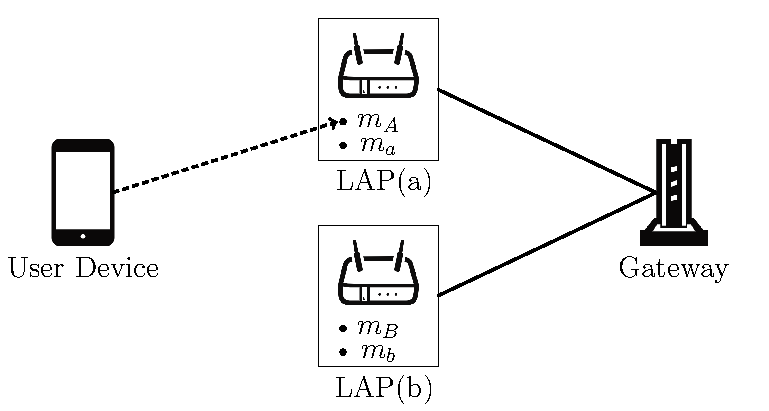
\includegraphics[scale=0.64]{starbucks/starbucks.pdf}
        \caption{The Network Model in the Cafe}
        \label{fig:sbx}
    \end{center}
    \vspace{-1zh}
\end{figure}
\begin{table}[t] 
    \begin{center}
        \caption{Evaluation Result in Real Environment}
        \label{tab:real}
        \begin{tabular}{c c} \hline
            ACC (\%) & Avg. Total Time (s) \\ \hline \hline
            100.0 & 32.1 \\ \hline
        \end{tabular}
    \end{center}
    \vspace{-2zh}
\end{table}

\tablename~\ref{tab:real} shows the results in the real environment.
The proposed scheme realizes 100\% accuracy even in real environment.
At that time, $\rm T$ is 32.1 seconds.
It is much shorter than the time that the most of recent security softwares take to scan their disk.
Thus, the safety of the LAN is guaranteed without being annoyed.
Through this result, we conclude the proposed scheme can accurately detect the attack with relatively short time in real LAN whose traffic is unstable.

However, as with other existing schemes, this work assumes Wi-Fi network models where Legitimate Repeaters (LR) are not installed.
It may be usual to introduce a LR in network to relay traffic farther at the expense of transmission speed in a large area.
In this case, the proposed scheme cannot distinguish a RAP and LR since both of them relay packets between a client and a LAP in the same way as MITM attack.
In order to detect the attack even in such Wi-Fi networks, we focus on their RSSI values as supplementary features because it can tell their general distance each other \cite{rssi}.
Since a LR has a function to relay packets from a LAP to devices which cannot connect with the LAP because of the long distance, it should be located far from a LAP in general.
In contrast, a RAP is basically introduced near a connecting LAP not to cause traffic delay due to their long distance.
Thus, we assume that an AP can be judged whether it is a LR or not on the basis of this idea.
In the future, we plan to devise the additional countermeasures and conduct some experiments so as to distinguish LR with RSSI value.

\section{Conclusion}\label{sec:6}
In this paper, we have proposed RAP detection by using ARP failure under the MAC address duplication.
We collect MAC addresses from user side and set the MAC address of a client to them.
By observing ARP packets in the situation, we can reveal the benignancy of the connected AP.
The detection performance of the proposed scheme is better than that of the previous scheme.
The results show it can detect a RAP without any error even in unstable traffic environment.
In addition, the experiment in a small cafe shows the availability in a real network.
In the future, we will conduct a large-scaled examination of the proposed scheme.
Furhermore, we will expand the scheme for the network where a LR is arranged.

\section{Acknowledgment}
This work is partly supported by the Grant in Aid for Scientific Research (No.17K06440) from Japan Society for Promotion of Science (JSPS).

%\bibliographystyle{ieicetr}% bib style
%\bibliography{}% your bib database
%\begin{thebibliography}{99}% more than 9 --> 99 / less than 10 --> 9
%\bibitem{}
%\end{thebibliography}
\bibliographystyle{IEEEtran}
\bibliography{IEEE_ref}
\vspace{12pt}
\profile{Kosuke Igarashi}{was born in Hokkaido, Japan in 1996. He received his B.S. degree from Keio University in 2020. He is a master student at Keio University. His research interest is security \& privacy for wireless communication.}
\profile{Hiroya Kato}{was born in Gunma, Japan in 1994. He received his M.S degree from Keio University in 2019. He is a Ph.D student at Keio University. His research interest is security \& privacy for IoT. He is a member of IEICE and IEEE.}
\profile{Iwao Sasase}{was born in Osaka, Japan in 1956. He received the B.E., M.E., and D.Eng. degrees in Electrical Engineering from Keio University, Yokohama, Japan, in 1979, 1981 and 1984, respectively. From 1984 to 1986, he was a Post Doctoral Fellow and Lecturer of Electrical Engineering at theUniversity of Ottawa,ON, Canada. He is currently a Professor of Information and Computer Science at Keio University, Yokohama, Japan. His research interests include modulation and coding, broadband mobile and  wireless communications, optical communications, communication networks and information theory. He has authored more than 297 journal papers and 445 international conference papers. He granted 45 Ph.D. degrees to his students in the above field. Dr. Sasase received the 1984 IEEE Communications Society (ComSoc) Student Paper Award (Region 10), 1986 Inoue Memorial Young Engineer Award, 1988 Hiroshi Ando Memorial Young EngineerAward, 1988 Shinohara MemorialYoung EngineerAward, 1996 Institute of Electronics, Information, and Communication Engineers (IEICE) of Japan Switching System Technical Group Best Paper Award, and WPMC2008 Best Paper Award. He is now serving as a President of IEICE. He served as President of the IEICE Communications Society (2012-2014). He was Board of Governors Member-at-Large (2010-2012), Japan Chapter Chair (2011-2012), Director of the Asia Pacific Region (2004-2005), Chair of the Satellite and Space Communications Technical Committee (2000-2002) of IEEE ComSoc., Vice President of the Communications Society (2004-2006), Chair of the Network System Technical Committee (2004-2006), Chair of the Communication System Technical Committee (2002-2004) of the IEICE Communications Society, Director of the Society of Information Theory and Its Applications in Japan (2001-2002). He is Fellowof IEICE, and Senior Member of IEEE, Member of the Information Processing Society of Japan.}
%\profile{}{}
%\profile*{}{}% without picture of author's face

\end{document}
